\graphicspath{{../Graphics/Cpt2-InjectCW/}}

En este c\'apitulo se ha estudiado la creci\'on de OFC mediante inyecci\'on de luz en funci\'on de las condiciones de la inyecci\'on, dadas por la potencia inyectada $P_{Iny}$ y la diferencia de frecuencias $\delta \nu$ entre la frecuencia del l\'aser maestro y el l\'aser esclavo (ML y SL respectivamente por sus siglas en ingl\'es). Se ha trabajado con el l\'aser ML en corriente continua con $\ibias = 35$ mA, $V_{RF} = 0$ V y $f_R = 5.0$ GHz.

Se han obtenido los diferentes r\'egimenes din\'amicos de los OFC en funci\'on de $P_{Iny}$ para dos valores de $\delta\nu$ distintos, uno positivo que equivale a una frecuencia de SL menor que la de ML, y otro negativo con el caso contrario.

En la Figura \ref{Img:zonasIO} se muestran los espectros \'opticos de las diferentes regiones din\'amicas obtenidas en funci\'on de $P_{Iny}$ para $\delta\nu = -2$ GHz. Se indica la frecuencia de inyecci\'on $\nu_{SL}$ con una flecha. 

			\begin{figure}[H]
				\centering
				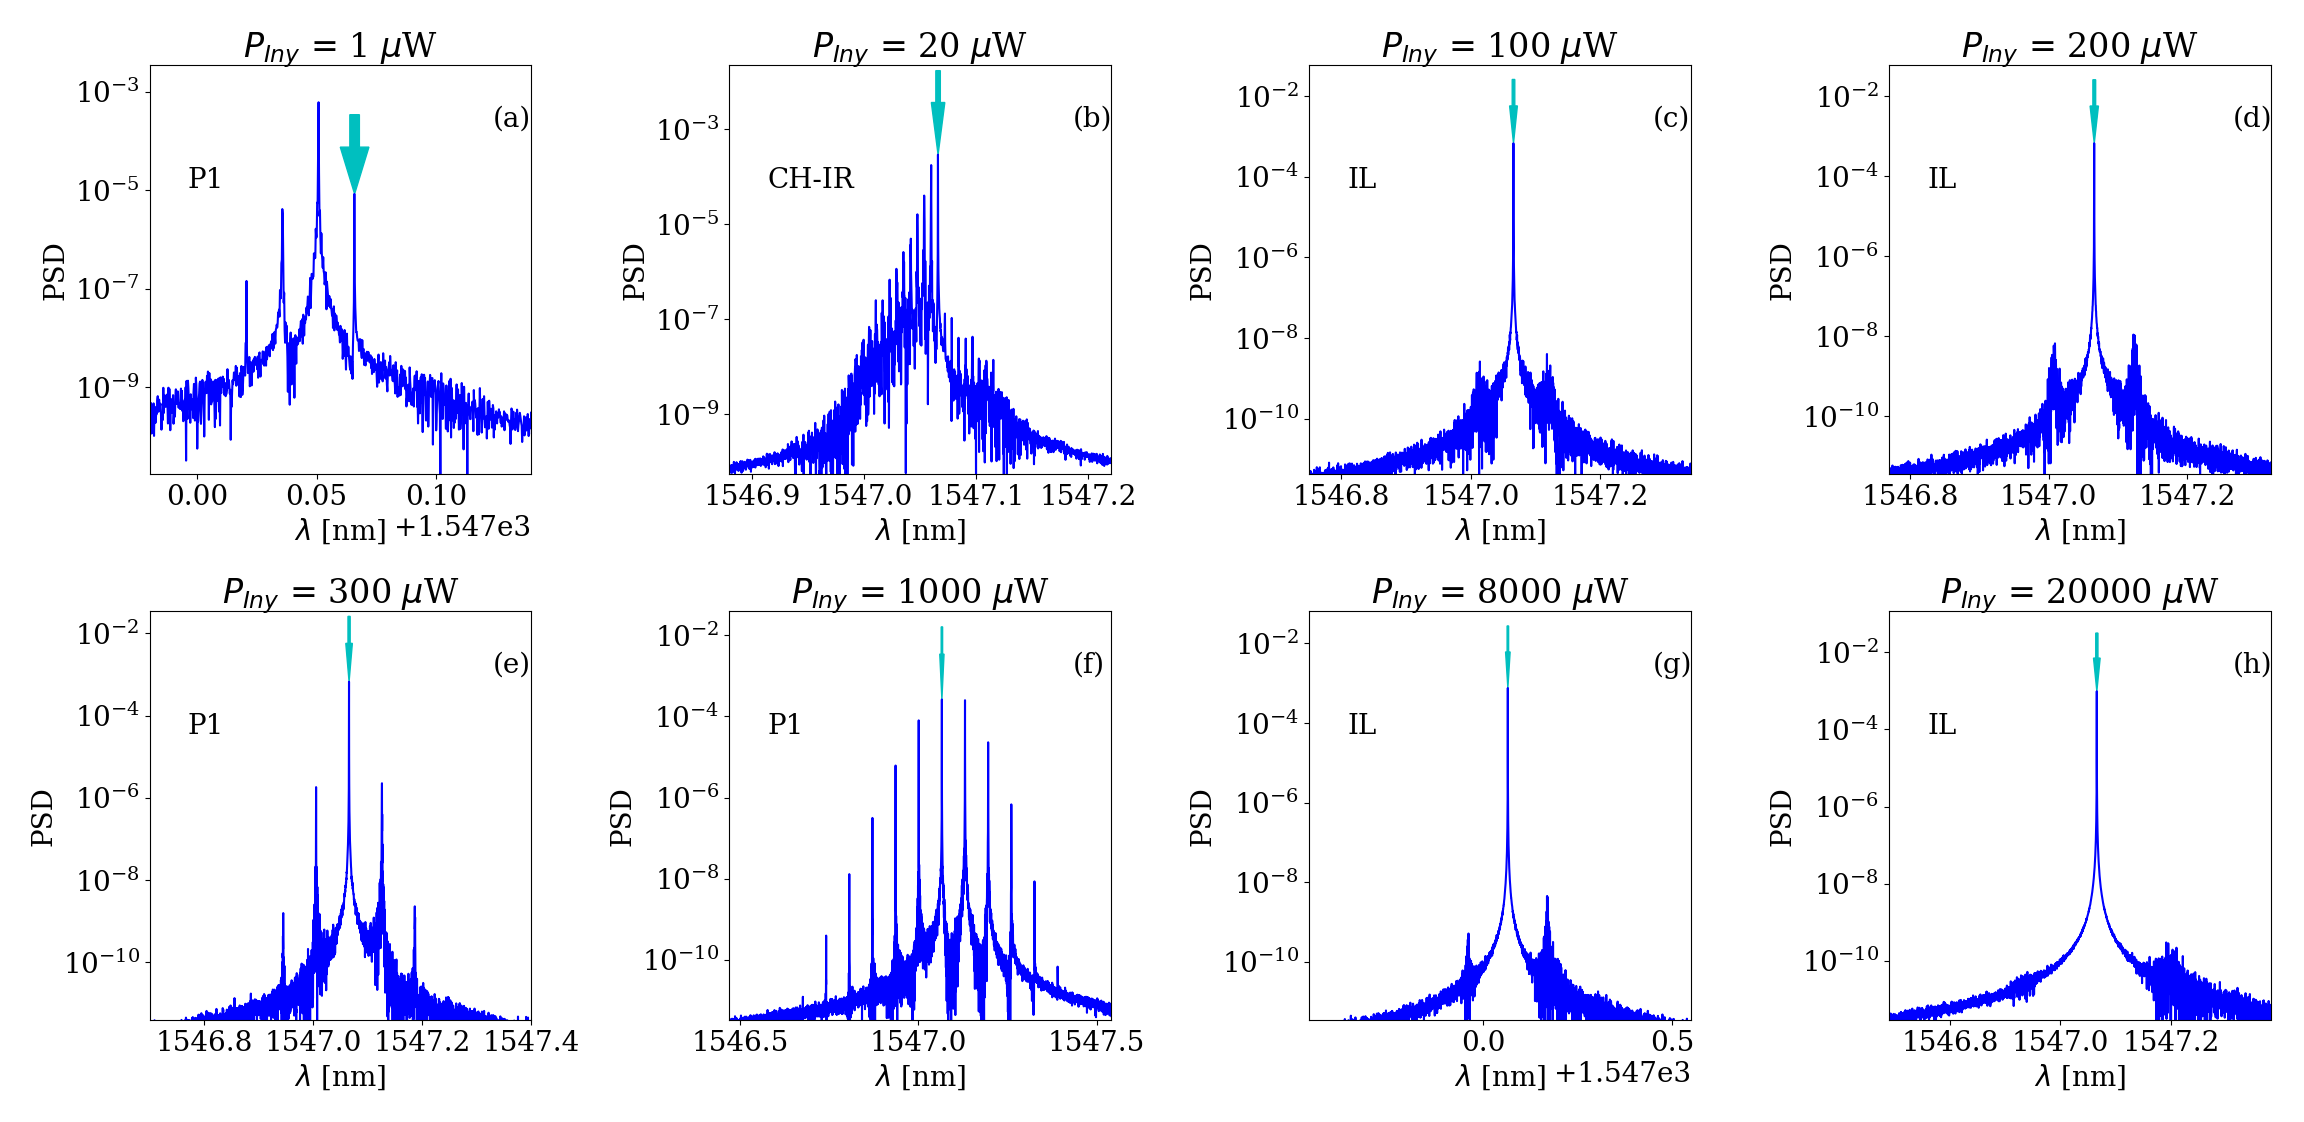
\includegraphics[width=1.0\linewidth]{zoneMap.png}
				\caption{\label{Img:zonasIO}Espectros \'opticos de las diferentes regiones din\'amicas obtenidas en funci\'on de $P_{Iny}$ para $\delta\nu = -2$ GHz. Se indica la frecuencia de inyecci\'on $\nu_{SL}$ con una flecha.}
			\end{figure}

		Para una baja potencia de inyecci\'on $P_{Iny} = 1 \; \mu$W (Figura \ref{Img:zonasIO} (a)) se obtiene un espectro \'optico con el pico de emisi\'on de ML y dos picos estimulados para la frecuencia de inyecci\'on $\nu_{SL}$. En esta regi\'on denominada de periodo 1, P1, las variables internas del \'aser logran estabilizarse \cite{vainio2006diode} debido a un fen\'omeno de \textit{Four-wave mixing} (FWM, mezcla de cuatro ondas). Al aumentar $P_{Iny}$ se llega a una regi\'on de caos, CH-IR ($P_{Iny} = 20\; \mu$W, Figura \ref{Img:zonasIO} (b)), con un OFC formado por muchas l\'ineas y con un perfil irregular. Esta regi\'on de caos se destruye para $P_{Iny} = 100\;\mu$W, en la que se obtiene un espectro \'optico con una \'unica l\'inea de emisi\'on para la frecuencia de inyecci\'on $\nu_{SL}$. Al aumentar la potencia de SL el l\'aser bloque la emisi\'on en $\nu_{ML}$ pasando a emitir solo en $\nu_{SL}$. A este fen\'omeno se le conoce como Bloqueo de Inyecci\'on (IL por sus siglas en ingl\'es). En la Figura \ref{Img:zonasIO} (d) se muestra el espectro para $P_{Iny} = 200\;\mu$W en IL, observando com al aumentar la potencia de inyecci\'on se empiezan a estimular las frecuencias de las oscilaciones de relajaci\'on. Esto ind\'ica que nos encontramos en el l\'imite de la regi\'on IL, encontrando una bifurcaci\'on de Van't Horf. Si se contin\'ua aumentando la potencia de inyecci\'on aumentar\'an los picos de la frecuencia de oscilaciones de relajaci\'on, retornando a la regi\'on P1 ($V_{RF} = 300\;\mu$W, Figura \ref{Img:zonasIO} (e)). Dentro de la refi\'on P1, el aumento de la potencia de inyecci\'on produce la aparici\'on de nuevas l\'ineas de emisi\'on, creciendo el OFC. Para altas potencias de inyecci\'on, $P_{Iny} = 8000 \;\mu$W y $20000 \;\mu$W, se regresa a la regi\'on IL.

		A partir de los datos experimentales \cite{Chaves19} se ha obtenido un mapa con las diferentes regiones din\'amicas en funci\'on de $P_{Iny}$ y $\delta\nu$. En la Figura \ref{fig:map} se muestra el mapa de las regiones din\'amicas obtenido a partir de \cite{Chaves19}, marcando los putos correspondientes a los espectros \'opticos de la Figura \ref{Img:zonasIO}.

			\begin{figure}[H]
				\centering
				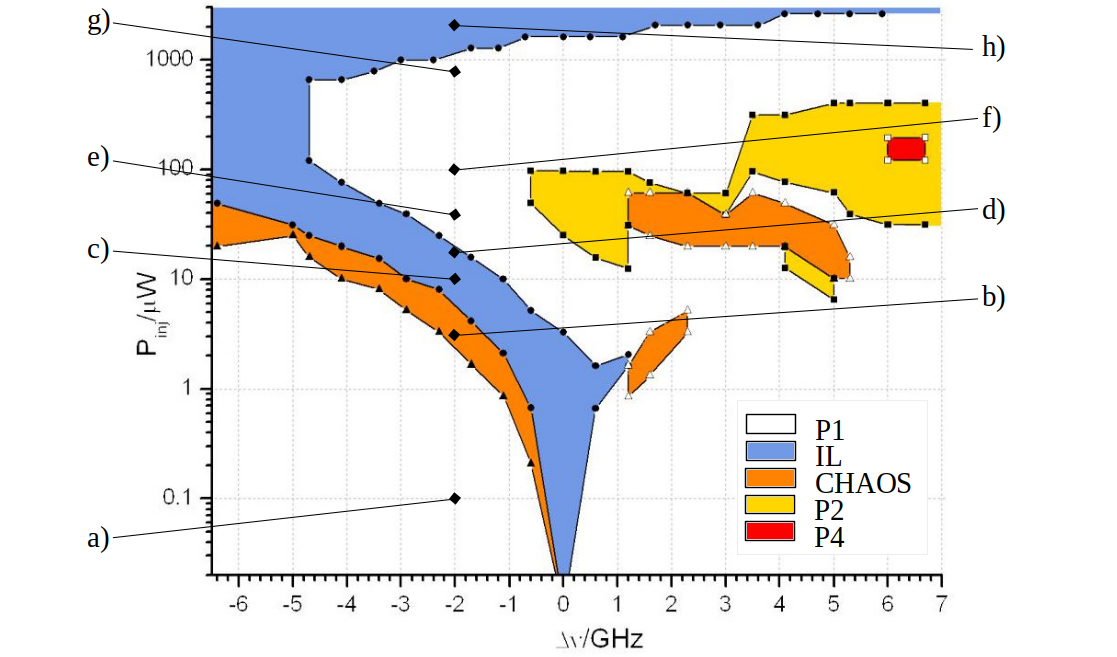
\includegraphics[width=0.7\linewidth]{maps.png}
				\caption{\label{fig:map}Mapa con las diferentes regiones din\'amicas en funci\'on de $P_{Iny}$ y $\delta\nu$ obtenido a partir de \cite{Chaves19}. Se han marcando los putos correspondientes a los espectros \'opticos de la Figura \ref{Img:zonasIO}.}
			\end{figure}

		Las regiones din\'amicas del mapa de la Figura \ref{fig:map} obtenidas experimentalmente, para las condiciones de inyecci\'on de los espectros \'opticos de la Figura \ref{Img:zonasIO} corresponden a las regiones obtenidas del an\'alisis de los resultados de la simulaci\'on.

		En la Figura \ref{fig:zoneRtEq} se muestran la potencia $P(t)$, la fase \'optica $\Phi (t)$ y el espectro \'optico de los tres casos m\'as representativos de la Figura \ref{Img:zonasIO} para cada regi\'on din\'amica obtenida: CH-IR, IL y P1. Esto permite estudiar los procesos que tienen lugar en las tres regiones encontradas para $\delta\nu = -2$ GHz. 

			\begin{figure}[H]
				\centering
				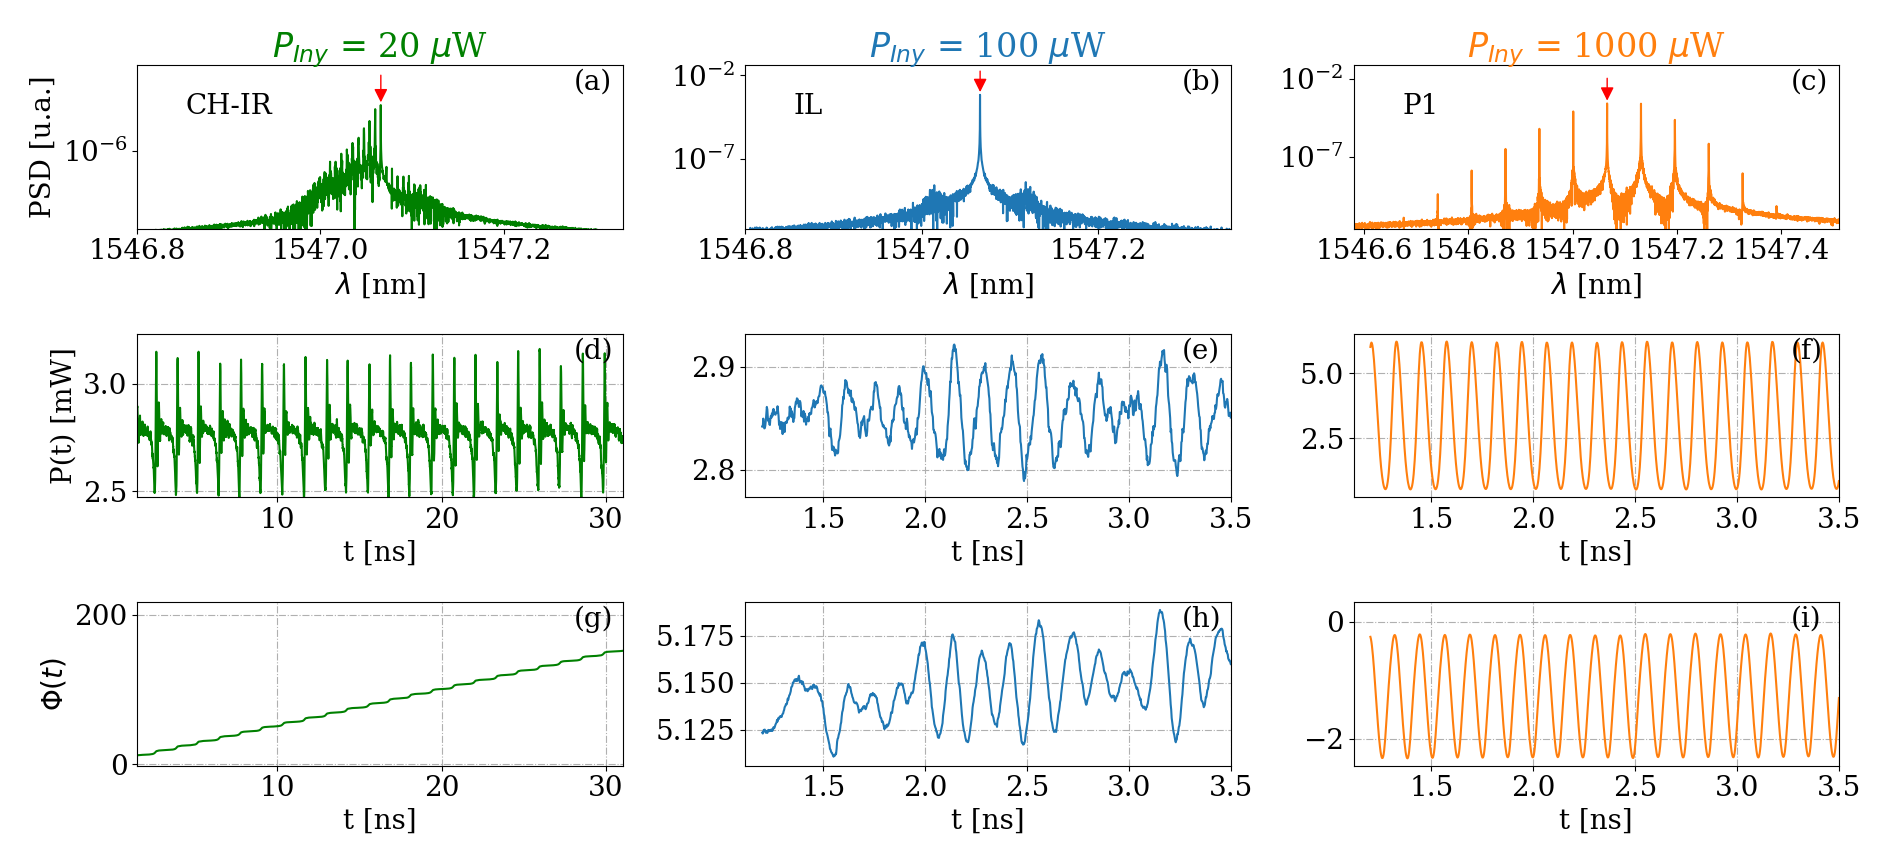
\includegraphics[width=1.0\linewidth]{zoneRtEq.png}
				\caption{\label{fig:zoneRtEq}Potencia $P(t)$, fase \'optica $\Phi (t)$ y espectro \'optico de los tres casos m\'as representativos de la Figura \ref{Img:zonasIO} para cada regi\'on din\'amica obtenida: CH-IR con $P_{Iny} = 20\;\mu$W (verde), IL con $P_{Iny} = 100\;\mu$W (azul) y P1 con $P_{Iny} = 1000\;\mu$W (naranja). Se indica en los espectros la frecuencia de inyecci\'on $\nu_{SL}$ con una flecha.}	
			\end{figure}

		Para el caso con $P_{Iny} = 1000\;\mu$W de la rigi\'on P1 se obtiene un espectro \'optico (Figura \ref{fig:zoneRtEq} (c)) se obtiene un OFC de buena calidad formado por varias l\'ineas bien resueltas y con las misma serparaci\'on entre ellas. Los perfiles temporales que se obtienen para $P(t)$ y $\Phi(t)$ son oscilaciones con una amplitud y periodo bien definidos, mostrando la estabilizaci\'on debida al FWM. En la Figura \ref{fig:zoneRtEq} (e)  se muestra el perfil temporal de la potencia para $P_{Iny} = 100\;\mu$W IL, que toma valores cercanos a un valor constante, realizando variaciones aleatroria y pequeñas entorno a dicho valor. Esto mismo se observa para su fase \'optica (Figura \ref{fig:zoneRtEq} (h)) en la que se obtienen variaciones de $\Phi(t)$ tres ordenes de magnitud menores que para P1. Con $P_{Iny} = 20\;\mu$W se encuentra la regi\'on CH-IR, con un perfil temporal de $P(t)$ similar al de IL (Figura \ref{fig:zoneRtEq} (d)) pero con unas pequeñas oscilaciones anarm\'onicas en un periodo $T \approx 1.25$ ns. La fase \'otica en CH-IR (Figura \ref{fig:zoneRtEq} (g)) aumenta a medida que el tiempo avanza.

		Del mapa de regiones din\'amicas de la Figura \ref{fig:map} se deduce que para $\delta\nu$ positivo se ha de poder alcanzar regiones con doblamiento de periodo, P2. En la Figura \ref{fig:P2zone} se muestran los espectros \'opticos, $P(t)$ y el atractor en el espacio de estados de las ecuaciones de balance, despreciando los efectos de la fase \'optica; para $\delta\nu = 5$ GHz y $P_{Iny} = 50\;\mu \textrm{W, } 1000\;\mu\textrm{W y } 200\;\mu$W.

			\begin{figure}[H]
				\centering
				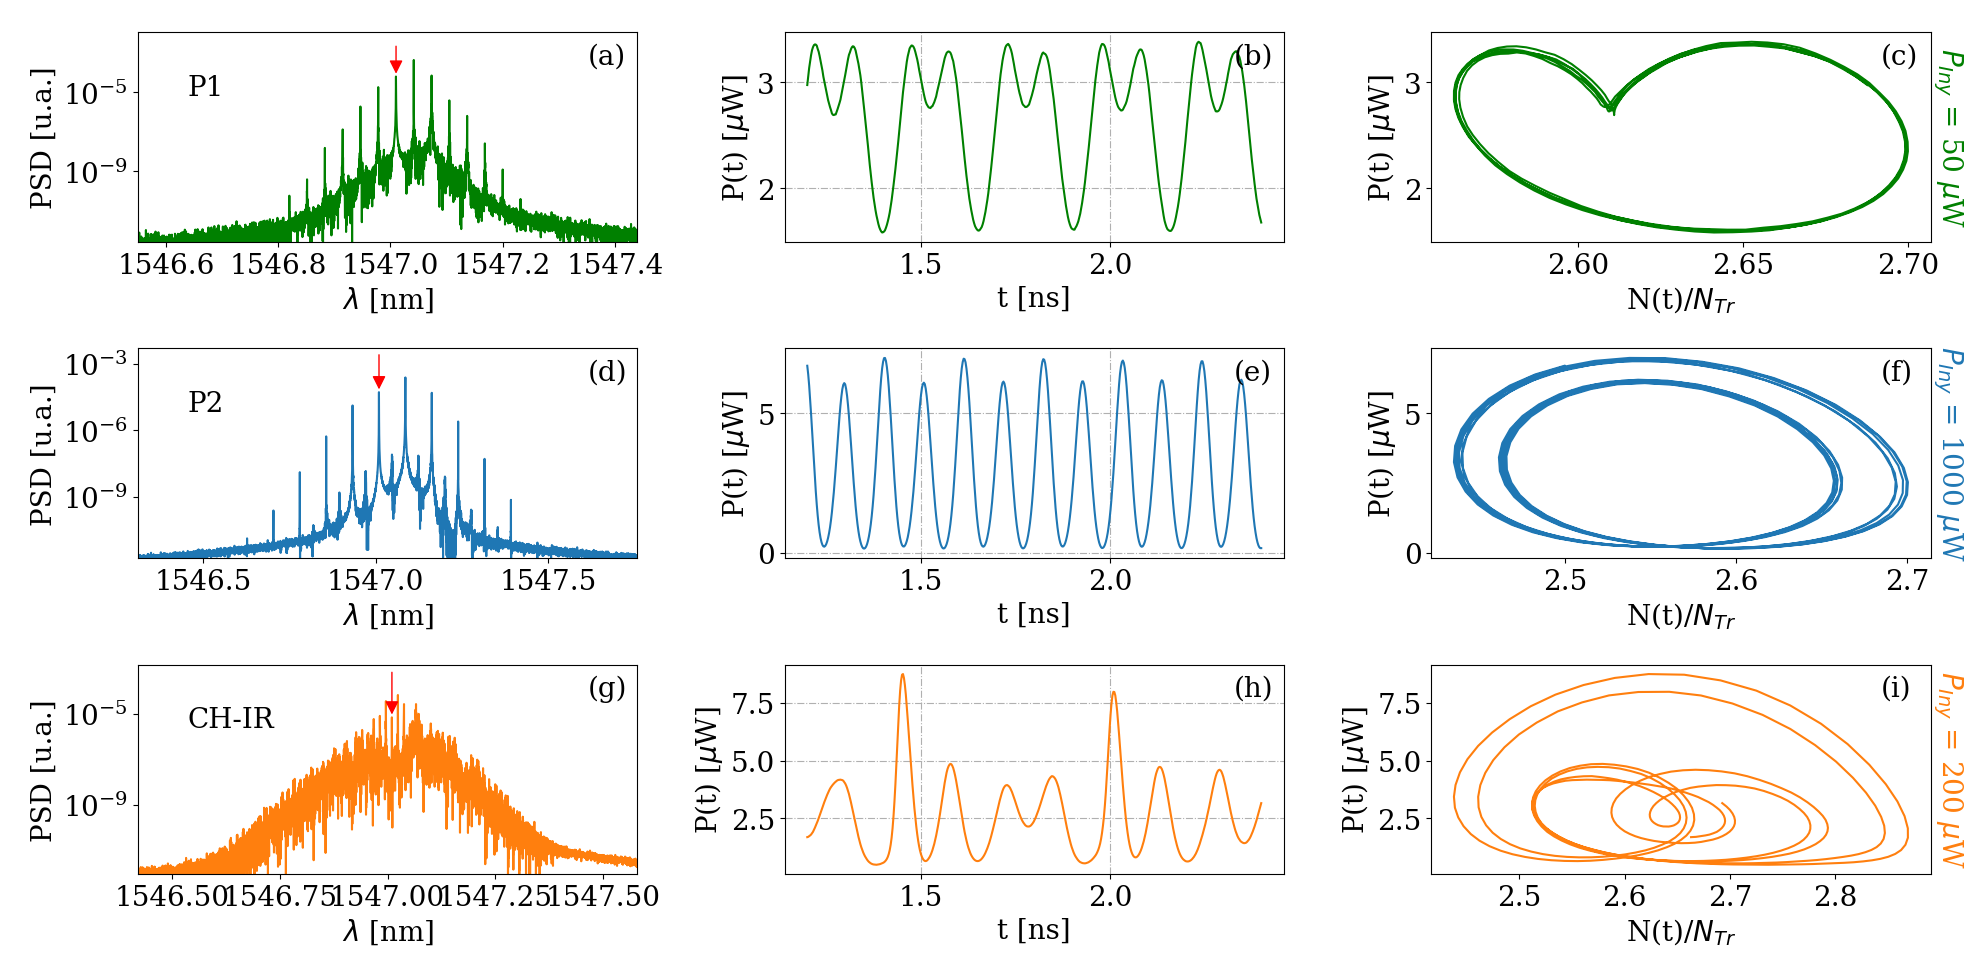
\includegraphics[width=1.0\linewidth]{P2zone.png}
				\caption{\label{fig:P2zone}Espectros \'opticos, $P(t)$ y atractor en el espacio de estados de las ecuaciones de balance, despreciando los efectos de la fase \'optica; para $\delta\nu = 5$ GHz y $P_{Iny} = 50\;\mu \textrm{W (verde), } 1000\;\mu\textrm{W (azul) y } 200\;\mu$W (naranja). Se indica en los espectros la frecuencia de inyecci\'on $\nu_{SL}$ con una flecha.}	
			\end{figure}

			Se obtiene de nuevo un OFC de buena calidad para la regi\'on P1 ($P_{Iny} = 50\;\mu$W, Figura \ref{fig:P2zone} (a)) y una $P(t)$ oscilante con una amplitud y frecuencia determinada (Figura \ref{fig:P2zone} (b)). Sin embargo, se observa como los m\'aximos de $P(t)$ comienzan a desdoblarse formando una segunda oscilaci\'on, indicando que se encuentra cerca de una regi\'on con doblamiento de periodo P2. \'Esto no se observa en el espectro \'optico debido a la poca intensidad de estos picos y al ruido debido a la emisi\'on espont\'anea, pero s\'i se puede ver en la Figura \ref{fig:P2zone} (c). El diagrama no llega a realizar una revoluci\'on completa sino que se dobla hacia el interior en un determinado punto. Al llegar la regi\'on P2 ($P_{Iny} = 1000\;\mu$W) la potencia se ha desdoblado completamente (Figura \ref{fig:P2zone} (e)), alternando picos de mayor y menor potencia. En el espectro \'optico (Figura \ref{fig:P2zone} (d)) se obtienen l\'ineas de emisi\'on escitadas entre las que se te\'ian en P1. La frecuencia de separaci\'on entre las l\'ineas cae a la mitad $\Delta \nu' = \frac{\Delat\nu}{2}$ y as\'i el periodo es el doble. En la Figura \ref{fig:P2zone} (f) aparece una nueva oscilaci\'on de menor amplitud debido al desdoblamiento de $P(t)$ y $N(t)$.

		Se alcanza la regi\'on CH-IR para $P_{Iny} = 200\;\mu$W, obteniendo un perfil de $P(t)$ con oscilaciones aleatrorias y sin una amplitud o frecuencia determinada (Figura \ref{fig:P2zone} (h)).El OFC del espectro \'optico (Figura \ref{fig:P2zone} (g)) se destruye completamente y el diagrama de estados de la Figura \ref{fig:P2zone} (i) describe una trayectoria irregular que para rangos de tiempo suficientemente grandes cubrir\'ia todo el espacio. 

		En la Figura \ref{fig:maps2} se muestra el mapa de las regiones din\'amicas obtenido a partir de \cite{Chaves19}, marcando los puntos correspondientes a las condiciones de inyecci\'on de los resultados de la Figura \ref{fig:P2zone}, obteniendo las mismas regiones que mediante el an\'alisis de los resultados de la simulaci\'on.

			\begin{figure}[H]
				\centering
				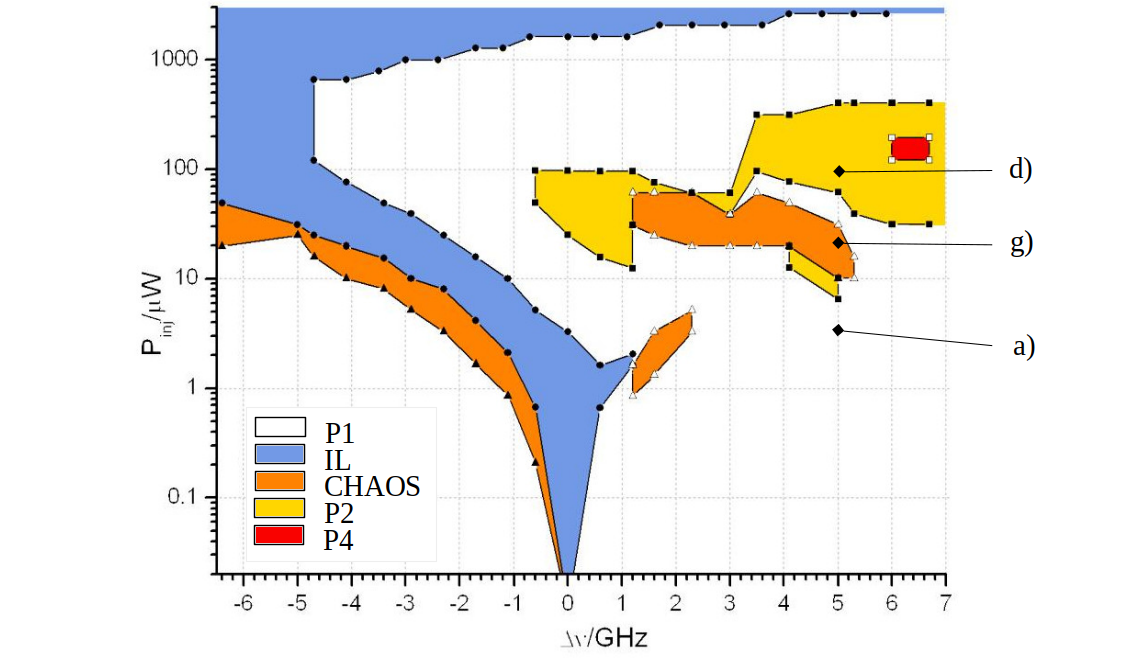
\includegraphics[width=0.7\linewidth]{maps2.png}
				\caption{\label{fig:maps2}Mapa con las diferentes regiones din\'amicas en funci\'on de $P_{Iny}$ y $\delta\nu$ obtenido a partir de \cite{Chaves19}. Se han marcando los putos correspondientes a las condiciones de inyecci\'on de la Figura \ref{fig:P2zone}.}	
			\end{figure}
